
\documentclass[12pt]{article}
\usepackage{geometry} % see geometry.pdf on how to lay out the page. There's lots.
\usepackage{graphicx}
\geometry{a4paper} % or letter or a5paper or ... etc
% \geometry{landscape} % rotated page geometry

% See the ``Article customise'' template for come common customisations

\title{MADAI Workbench 1.8.0 Tutorial: \\A Supplement to the ParaView Tutorial}
\author{Cory Quammen}
\date{} % delete this line to display the current date

%%% BEGIN DOCUMENT
\begin{document}

\maketitle
\tableofcontents

\section{Introduction}

This tutorial will walk you through using several of the features of the MADAI Workbench. These features not available in a plain installation of ParaView.

The content of this tutorial assumes that you have gone through the ParaView Tutorial for version 3.98 or higher of ParaView.

\section{Ensemble Surface Slicing Representation}

In the ParaView tutorial, we have seen that several representations are available for displaying data in ParaView (3D Glyphs, Outline, Points, Surface, Surface with Edges, Wireframe). Another representation is suitable for displaying a group of surfaces using a technique called Ensemble Surface Slicing \cite{Oluwafemi2012}.

Open the files \texttt{apple.ply}, \texttt{banana.ply}, \texttt{cherry.ply}, and \texttt{grape.ply}. The Ensemble Surface Slicing representation operates on a set of surfaces grouped together into a multiblock dataset. To group the files, select them all in the Pipeline Browser by holding the shift key and selecting the first file in the browser and then the last. Next, group them together with Filters $\rightarrow$ Alphabetical $\rightarrow$ Group Datasets. The resulting display will show the union of the surfaces, the same as what you would get just by having all the surfaces' visibility turned on.

\begin{figure}[htbp]
   \centering
   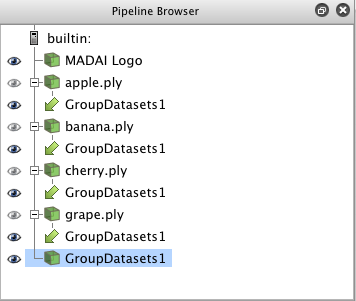
\includegraphics[scale=.5]{images/ESSGroupDatasets.png} % requires the graphicx package
   \caption{The fruit datasets \texttt{apple.ply}, \texttt{banana.ply}, \texttt{cherry.ply}, and \texttt{grape.ply} grouped together.}
   \label{fig:ESSGroupDatasets}
\end{figure}

Next, change the representation of the grouped surfaces to \textbf{Ensemble Surface Slicing}. Change the \textbf{Slice Width} setting to 2 and the \textbf{Plane Normal} to 0, 0, 1. You will now see all the surfaces, but slices will be taken out of each surface in such a way that shows all the surfaces.

\begin{figure}[htbp]
   \centering
   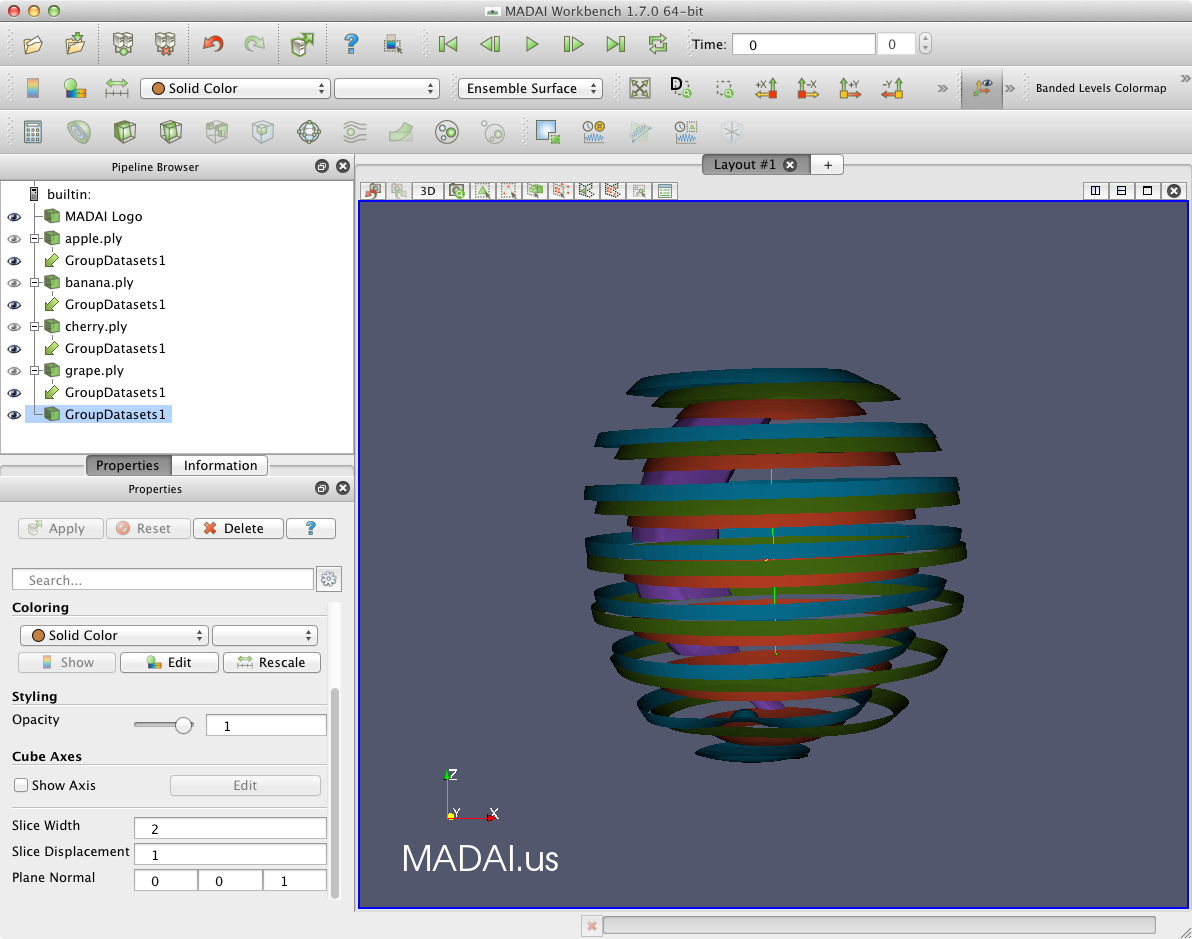
\includegraphics[scale=.25]{images/ESSSurfaces.png} % requires the graphicx package
   \caption{The fruit datasets displayed with the ensemble surface slicing technique.}
   \label{fig:ESSSurfaces}
\end{figure}

\section{Threshold Points Filter}

ParaView provides a Threshold filter that operates on cells in a dataset. Cells, such as triangle or tetrahedra, are elements that either have a surface area or volume. This is a problem when your dataset consists of points with no associated cells. This can show up in strange ways when you have applied a Threshold filter to your dataset, but no filtering appears to have been done.

To see that this is the case, create a point source by selecting Sources $\rightarrow$ Point Source. Change the \textbf{Number of Points} to 1000 and \textbf{Radius} to 1. Next, create a \textbf{Calculator} filter by selecting \textbf{Filters} $\rightarrow$ \textbf{Alphabetical} $\rightarrow$ \textbf{Calculator}. Set the \textbf{Result Array Name} to ``X'' and enter ``coordsX'' in the text field above the calculator buttons. This creates a point scalar field that has the same value as the x-coordinates of the points.

\begin{figure}[htbp]
   \centering
   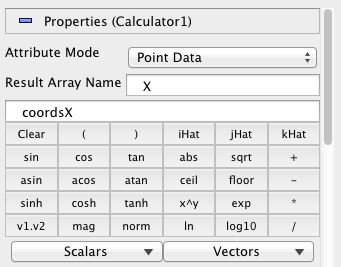
\includegraphics[scale=.5]{images/ThresholdPointsFilterCalculator.png} % requires the graphicx package
   \caption{Creating a point scalar field for the point data.}
   \label{fig:PointsFilterCalculator}
\end{figure}

No apply the Threshold filter (Filters $\rightarrow$ Alphabetical $\rightarrow$ Threshold). Select ``X'' from the \textbf{Scalars} menu and uncheck the \textbf{All Scalars} checkbox and then click \textbf{Apply}. You should see all the original points. Next, change the \textbf{Maximum} value to 0.2. Again, all the original points are displayed, indicating that thresholding did not work. Select the \textbf{Calculator1} filter in the Pipeline Browser again and this time create a Threshold Points filter (Filters $\rightarrow$ Alphabetical $\rightarrow$ Threshold Points Filter). Select ``X'' as the scalars and change the right value of the \textbf{Threshold Range} to 0.2. This time, the points will be filtered such that points with the X value (and x-coordinate) above 0.2 are removed from the point set.

\begin{figure}[htbp]
   \centering
   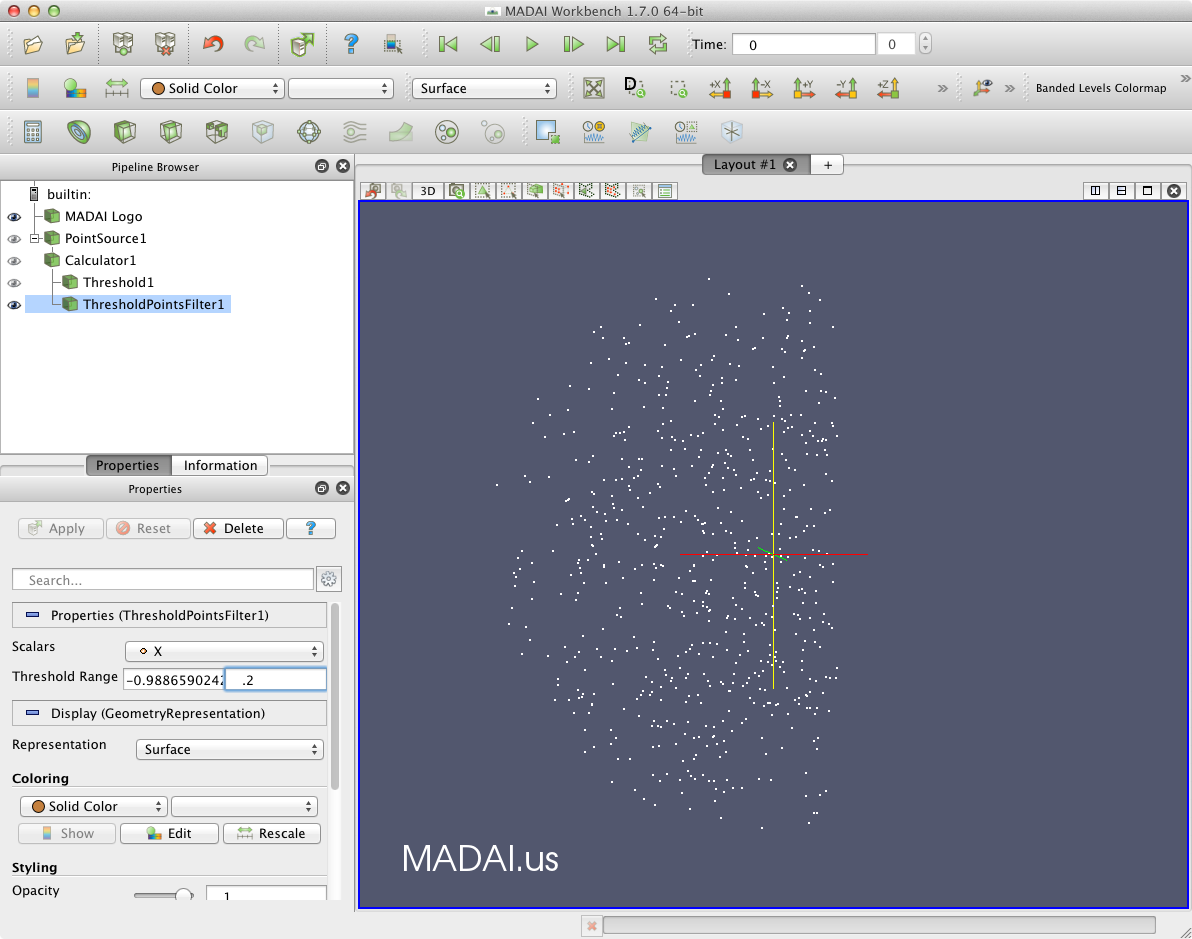
\includegraphics[scale=.25]{images/ThresholdPointsFilter.png} % requires the graphicx package
   \caption{Results of the \textbf{Threshold Points} filter.}
   \label{fig:PointsFilterCalculator}
\end{figure}

\section{Binning Filter}


\section{Gaussian Scalar Splatter Filter}

\section{}

\bibliographystyle{plain}
\bibliography{MADAIWorkbenchTutorial}

\end{document}